\chapter{Introduction}
\graphicspath{{foto/Chap1/}}
\section{Introduction to the laboratory experience}
This project aims to estimate the characteristics of a 3D NAND memory array based on Traditional Planar Transistors through a MATLAB script.

The outputs of the model are:
\begin{itemize}[noitemsep, topsep=0pt]
\item Delay during a precharge and read operation
\item Power consumption due to a read operation
\item Power consumption due to a write operation
\item Power consumption due to an erase operation
\item Area and Volume
\end{itemize}

\section{Structure explanation}
The 3D NAND memory exploits the vertical dimension to increase the bit density of the array. From a logical point of view, the model is represented by a series of memory blocks called "slices" that together form the array, as shown in fig. \ref{fig:memory}. Every slice works like a traditional planar NAND memory block. So, after selecting a slice, the behaviour of the memory is the same as a planar one. All around the memory slices there are some pieces of circuit (Decoders) used to select the desired memory cell, plus other circuits, like Sense Amplifiers and Precharge Units, as shown in fig. \ref{fig:3dmemory}.

\begin{figure}[H] 
	\begin{center}
		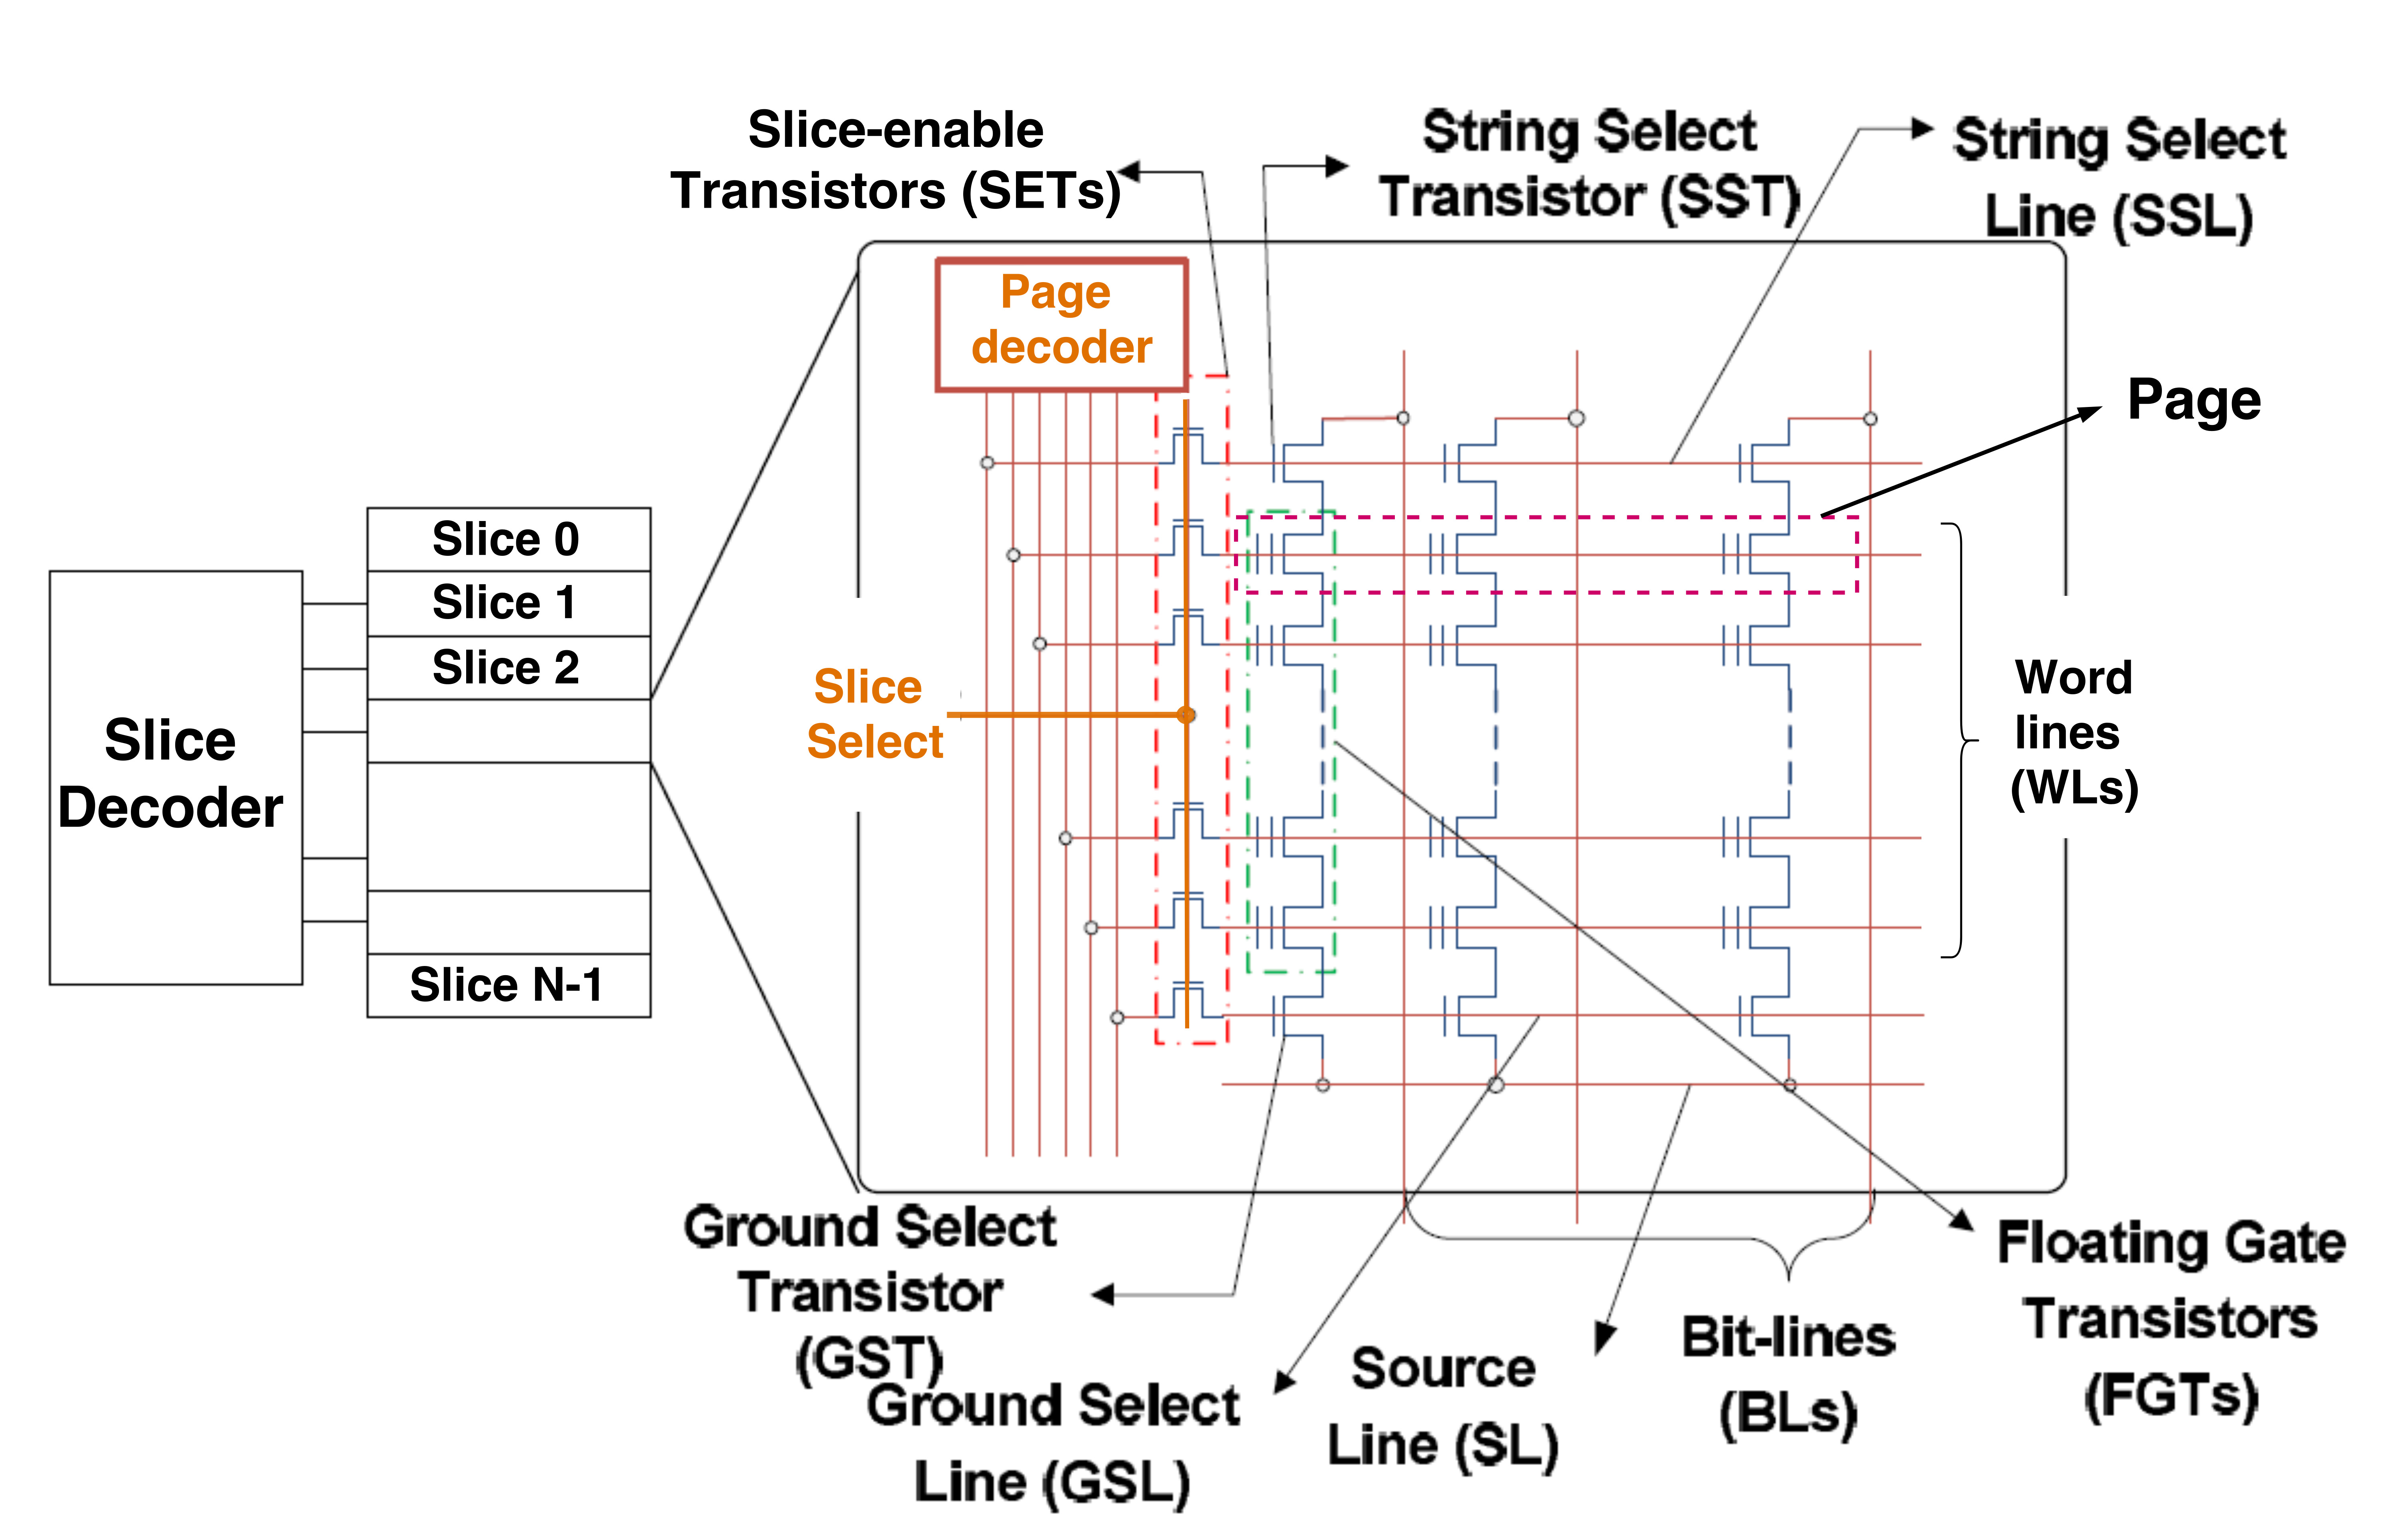
\includegraphics[width=0.85\textwidth]{memory}
	\end{center}
	\caption{Block structure of the memory} 
	\label{fig:memory}
\end{figure} 

The elements that dissipate energy are:

\begin{itemize}
\item String select line (SSL)
\item Ground select line (GSL)
\item Bitlines (BLs)
\item Wordlines (WLs)
\item Slice enable transistors (SETs)
\item String select transistor (SST)
\item Ground select transistor (GST)
\item Floating gate transistors (FGTs)
\end{itemize}

\begin{center}
	\begin{figure}[H]
		\centering
		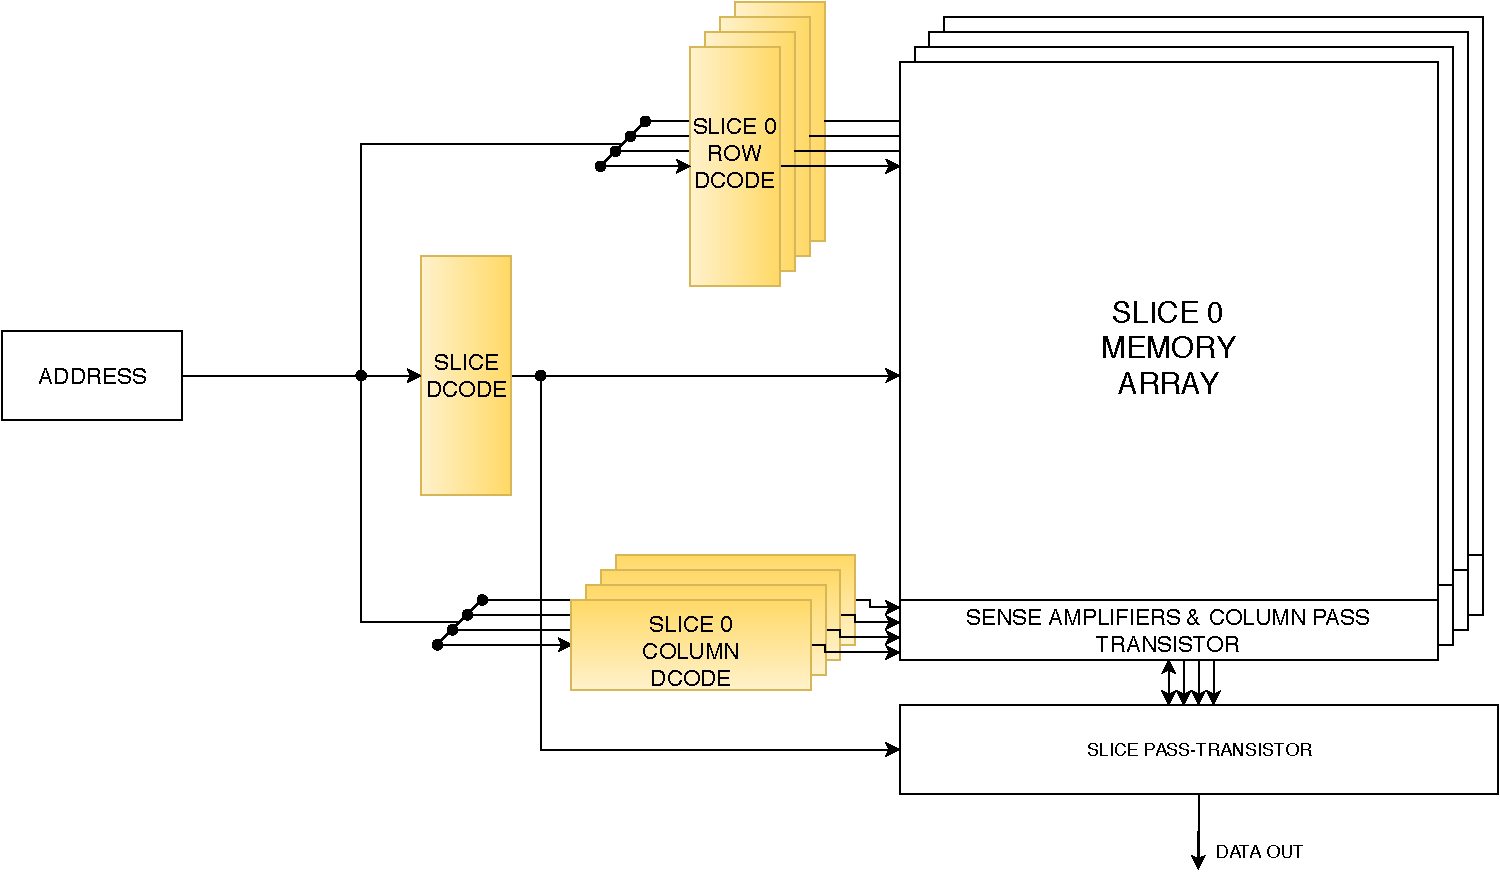
\includegraphics[scale = 0.55]{3dmemory-GENERAL_SCHEMATIC}
		\caption{Block diagram of the total structure}
		\label{fig:3dmemory}
	\end{figure}
\end{center}

\section{Behavior of the memory}
The behaviour of the memory can be modelled like a FSM with these states, as shown in fig. \ref{fig:fsm}:

\begin{itemize}[noitemsep, topsep=0pt]
\item Precharge
\item Read
\item Write
\item Erase
\end{itemize}

\begin{center}
	\begin{figure}[H]
		\centering
		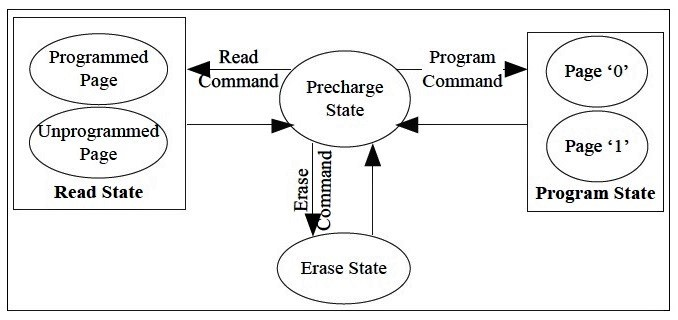
\includegraphics[scale = 0.6]{FSM}
		\caption{State machine for memory operation}
		\label{fig:fsm}
	\end{figure}
\end{center}

\textbf{Precharge} is the initial state to perform a \textbf{read}, \textbf{write} or \textbf{erase} operation. During the precharge state, bitlines are biased at a certain voltage to speed up subsequent operations. Bitlines are electrically disconnected from the memory array because the SSL signal is not asserted. Thanks to slice enable transistors (SETs), the wordlines are electrically disconnected too.

\textbf{Read} and \textbf{Write} operations are performed at page level while erase at slice level. During any operation, unselected slices are electrically disconnected by the slice decoder.\\

The memory array in standard planar NAND is obviously a plane but in 3D ones it has a cubic shape. The cube is organized in blocks that in the model are referred to as \textit{slices}. A slice decoder is used to select only the desired slice and to electrically isolate the others.

The layout is organized in rows (\textit{wordlines}) and columns (\textit{bitlines}). At the intersection of each row and column there is a Floating Gate Transistor (FGT) that is the actual memory element. In the project a SLC (single-level cell) flash is used so each FGT stores only one bit of data. The FGTs connected in series form a \textit{string} and can be accessed using the String Select Transistor (SST) and the Ground Select Transistor (GST). The group of FGTs along the same WL is called \textit{page} and it is selected using the page decoder.

Flash memory exploits Tunneling Effect to perform write/erase operations on the FGTs. The write operation moves the tunneling charges in the floating gate, while they are extracted from it during the erase phase.\\

The model of the memory incudes also all the peripheral components needed to select the bits and to read them: apart from the memory slices, so, we have modelled also the slice, the row and column decoders, the sense amplifiers and all the pass transistors needed for the correct selection of the lines and for providing the data towards the external world. The behaviour of each component during a read operation will be better detailed in chapter \ref{sec:Delay}.

We report in fig. \ref{fig:3dmemory_scheme} a more detailed scheme of the memory. We must remember that, being a flash memory, the data to be stored inside the chip is typically huge; for this reason each row of each slice will for sure have to host more than a single word. For example, we could consider a slice whose dimension is $1024\times1024$ bits: if a single word has 64 bits of parallelism, in each row we'll have 16 words stored.

\begin{center}
	\begin{figure}[H]
		\centering
		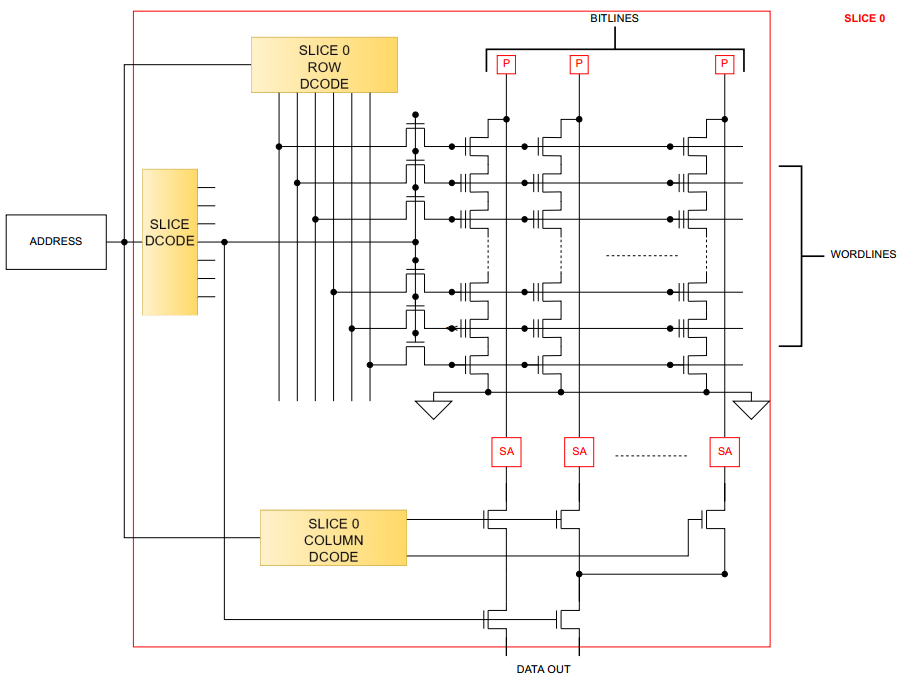
\includegraphics[scale = 0.6]{3dmemory-SLICE_SCHEME.png}
		\caption{Detailed memory scheme}
		\label{fig:3dmemory_scheme}
	\end{figure}
\end{center}

Let's say, to make a practical example which can be adapted to fig. \ref{fig:3dmemory_scheme}, that instead of 64 bits of parallelism, each word has only 2 bits. Then, in an array $1024\times1024$, we would have 512 words per row. After the activation of the corresponding wordline, all these 512 words will force the value of their bits on the 1024 bitlines. So the 1024 sense amplifiers will accelerate the detection of the stored value. However, the column decoder will allow only the correct couple out of these 512 couples to reach the drain of the two last pass transistors, which transmit the correct 2-bits read word to the external world.

The parameters provided in input to the model, then, are $N_{bl}$ (number of bitlines per slice), $N_{wl}$ (number of wordlines per slice), $N_{slice}$ (number of slices) and $N_{bit,word}$ (number of bits per word). The number of bits per address so are computed like:
$$Block\_Address=\left\lceil log_2(N_{slice})\right\rceil$$
$$Row\_Address=\left\lceil log_2(N_{wl})\right\rceil$$
$$Column\_Address=\left\lceil log_2\left(\frac{N_{bl}}{N_{bit,word}}\right)\right\rceil$$



